\chapter{Introduction to Novelty Detection}
\label{ch:GeneralND}

\begin{figure}
    \centering
    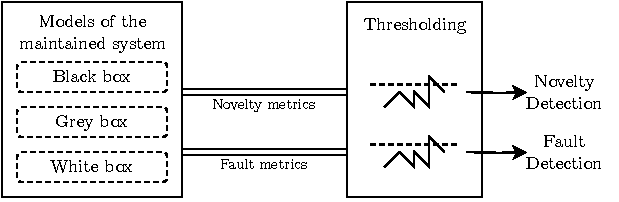
\includegraphics[width=\textwidth]{images/Intro/GeneralND.pdf}
    \caption{General working principle of Novelty Detection}
    \label{fig:IntroToND}
\end{figure}

This short chapter is dedicated to the introduction of the general working principles behind any kind of \gls{nd} or \gls{fd}. 

As already mentioned in the introduction and in \autoref{fig:MaintTriangle}, the models behind the study of the behaviour of a system are various. Often, in the field of \gls{nd}, the models rely on \gls{ml} rather than on a physical model. Sometimes, the model is based on a combination of both, as some physical knowledge is used to guide the \gls{ml} model.

Regardless of the model used, to perform \gls{nd} or \gls{fd} a measure of the deterioration of the system is needed. Then, the problem of deciding when to declare a novelty or a fault arises. All the models that rely on real data have to face the problem of noise. This unpredictability will cause some outliers in the detection. 

\paragraph{Thresholding}
\label{sec:Thresholding}

A common approach used to trigger the \gls{nd} or \gls{fd} warnings to the operator is to set a threshold on the measure of the deterioration. This principle is illustrated in \autoref{fig:IntroToND}. 

In the case of a physical model, the threshold can be decided by an expert in the field, as the degradation metric will be a physical measure. In the case of an \gls{ml} model, instead, the degradation measure will be harder to interpret in a physical way. 

In \autoref{ch:MachineLearning}, several \gls{ml} models will be described. For some of them, the measure of the deterioration will be a probability, for others, it will be a distance, for others, it will be density, and so on. So, in some cases, the deterioration metric can be interpreted in a geometric way, as in the case of K-means and \gls{dbscan}.

Using the geometric normalization, an educated guess of the threshold can be made. For example, in the case of K-means, the metric is the distance from the \gls{glo:cent} normalized by the radius of the \gls{glo:clust}, so a threshold of 1 would mean to consider anomalous a measure that is twice as far away from a \gls{glo:clust} \gls{glo:cent} \gls{wrt} the furthest known record.

Another common approach is to first see the distribution of the measure of the deterioration and then decide the threshold. This operation affects the false positive and false negative rates.

\paragraph{Approach used in this work}

Another problem arises when comparing the performance of different models. The real degradation of the system normally continues in time, so any model can be made to detect a novelty as soon as it is desired, by setting the threshold to a very low value. This is clearly not a fair comparison, because a bias is introduced in the act of deciding the threshold. To avoid that, a common approach to thresholding will be used among all the algorithms.

In this work, several models will be compared on the same datasets. For this reason, a common approach to thresholding will be used. The naive approach is to decide arbitrarily a time window in which the measure is considered normal. And set the threshold to a value that is higher than the maximum value of the measure in the time window. This approach is naive but, being used for all the models, this will reduce the bias in the comparison.